\documentclass[load-preamble]{cnltx-doc}
\usepackage[T1]{fontenc}
\usepackage[utf8]{inputenc}

\usepackage{filecontents}

\usepackage{imakeidx}
\begin{filecontents*}{\jobname.ist}
 heading_prefix "{\\bfseries "
 heading_suffix "\\hfil}\\nopagebreak\n"
 headings_flag  1
 delim_0 "\\dotfill"
 delim_1 "\\dotfill"
 delim_2 "\\dotfill"
 delim_r "\\textendash"
 delim_t ""
 suffix_2p "\\nohyperpage{\\,f.}"
 suffix_3p "\\nohyperpage{\\,ff.}"
\end{filecontents*}
\indexsetup{othercode=\footnotesize}
\makeindex[options={-s \jobname.ist},intoc,columns=3,columnsep=1em]

\setcnltxample{
  class = cnltxample ,
  subtitle = Documentation for \LaTeXe\ Packages or Classes ,
  info     = \LaTeX\ examples the \texorpdfstring{\textsc{cn}}{CN} way ,
  authors  = Clemens Niederberger ,
  email    = contact@mychemistry.eu ,
  url      = https://github.com/cgnieder/cnltxample ,
  abstract = {%
    A bundle of a package and a class for consistent format of control
    sequences, package options, source code with examples, writing a package
    manual (including an index containing the explained control sequences,
    options, \ldots).%
  } ,
  add-cmds = {
    code,codefont,command,cs,csidx,
    Default,default,
    env,environment,
    key,keybool,keychoice,keyval,
    marg,oarg,darg,sarg,
    opt,option,
    setcnltxample
  },
  add-envs = {
    commands,
    environments,
    example,
    options
  },
  add-frame-options = {
    innerleftmargin=2em
  }
}

\makeatletter
\def\cnltx{\cnltx@package@name@format{cnltx}}
\def\cnltxexample{\cnltx@package@name@format{cnltx-example}}
\def\cnltxdoc{\cnltx@package@name@format{cnltx-doc}}

\newrobustcmd\bypackage{%
  \cnltx@version@note{provided by the \cnltxexample\ package}%
}
\newrobustcmd\byclass{%
  \cnltx@version@note{provided by the \cnltxdoc\ class}%
}
\makeatother

\newcommand*\file[1]{\code{#1}}

% \usepackage{showframe}
% \usepackage{kantlipsum}

\begin{document}

\section{Background}

The \cnltx\ bundle contains of a package and a class both with the same
name.  I developed them as a successor of a class that I used for writing the
documentation of my packages with the intention of a cleaner interface and
less unnecessary ballast.  Hence the separation into package and class.  The
package provides a source code environment that also prints the output and
defines quite a number of macros for formatting of control sequence names,
package names, package options and so on.  The best documentation for the
bundle as always is the source code but I'm trying to provide a documentation
as comprehensive as possible.

\section{License and Requirements}\label{sec:license}
\license

The \cnltx\ package loads the following packages:
\pkg{etoolbox}\footnote{\CTANurl{etoolbox}},
\pkg{xcolor}\footnote{\CTANurl{xcolor}},
\pkg{pgfopts}\footnote{\CTANurl{pgfopts}},
\pkg{listings}\footnote{\CTANurl{listings}},
\pkg{trimspaces}\footnote{\CTANurl{trimspaces}},
\pkg{accsupp}\footnote{\CTANurl[macros/latex/contrib/oberdiek]{accsupp}},
\pkg{mdframed}\footnote{\CTANurl{mdframed}} and
\pkg{idxcmds}\footnote{\CTANurl{idxcmds}}.

The \cnltx\ class loads the package with the same name and additionally
the following packages: \pkg{ulem}\footnote{\CTANurl{ulem}},
\pkg{multicol}\footnote{\CTANurl[macros/latex/required/tools]{multicol}},
\pkg{ragged2e}\footnote{\CTANurl[macros/latex/contrib/ms]{ragged2e}},
\pkg{marginnote}\footnote{\CTANurl{marginnote}} and
\pkg{hyperref}\footnote{\CTANurl{hyperref}}. It is a wrapper class for the
\KOMAScript\ class \cls{scrartcl}\footnote{\CTANurl{koma-script}}.

Like all of my packages \cnltx\ implicitly relies on an up to date \TeX\
distribution.

\section{Options and Setup}
The \cnltx\ bundle has a number of options.  The package knows most of
them as package option, the class only knows the \option{load-preamble}
(described in section~\ref{sec:preamble}).  All options except the one class
option regardless if they're defined by the package or the class can be set
with a setup command:
\begin{commands}
  \command{setcnltxample}[\marg{options}]
    setup command for \cnltx.
\end{commands}
The source code environments also have optional arguments that can be used to
set the options for the environment locally.

\section{Available Commands}
\subsection{Description of Macros, Environments and  Options}\label{sec:cmds:macros}

The commands described in this section all are provided by the \cnltx\
package\bypackage.  They all are related to the typesetting of provided
macros, options and the like.

\begin{commands}
  \command{code}[\marg{arg}]
    Formatting of source code.  This is \emph{no} verbatim command.  Used
    internally in the following commands.
  \command{cs}[\sarg\marg{name}]
    Format the control sequence \meta{name}, \cs{cs}\code{\{name\}}:
    \cs*{name}.  Adds a corresponding index entry.  The starred form does not
    add an index entry.
  \command{csidx}[\marg{name}]
    Adds an index entry but does not typeset the control sequence
    \meta{name}.
  \command{env}[\sarg\marg{name}]
    Format the environment \meta{name}, \cs{env}\code{\{name\}}:
    \env*{name}.  Adds a corresponding index entry with a hint that the entry
    refers to an environment.  The starred form does not add an index entry.
  \command{envidx}[\marg{name}]
    Adds an index entry but does not typeset the environment \meta{name}.
  \command{meta}[\marg{meta}]
    Description of an argument, \cs{meta}\code{\{meta\}}: \meta{meta}.
  \command{marg}[\marg{arg}]
    A mandatory argument. \meta{arg} is formatted with \cs{meta} if it is not
    blank, \cs{marg}\code{\{arg\}}: \marg{arg}.
  \command{oarg}[\marg{arg}]
    An optional argument. \meta{arg} is formatted with \cs{meta} if it is not
    blank, \cs{oarg}\code{\{arg\}}: \oarg{arg}.
  \command{darg}[\marg{arg}]
    An argument with parentheses as delimiters. \meta{arg} is formatted with
    \cs{meta} if it is not blank, \cs{darg}\code{\{arg\}}: \darg{arg}.
  \command{sarg}
    An optional star argument, \cs{sarg}: \sarg.
  \command{option}[\sarg\marg{name}]
    An option \meta{name}, \cs{option}\code{\{name\}}: \option{name}.  Adds a
    corresponding index entry.  The starred form does not add an index entry.
  \command{optionidx}[\marg{name}]
    Adds an index entry but does not typeset the option \meta{name}.
  \command{key}[\sarg\marg{name}\marg{values}]
    A key \meta{name} with values \meta{values},
    \cs{key}\code{\{key\}}\code{\{value\}}: \key{key}{value};
    \cs{key}\sarg\code{\{key\}}\code{\{value\}}: \key*{key}{value}
  \command{choices}[\marg{clist of choices}]
    A list of choices, \cs{choices}\code{\{one,two,three\}}:
    \choices{one,two,three}
  \command{choicekey}[\marg{name}\marg{clist of choices}]
    A key \meta{name} with a list of possible values,
    \cs{choicekey}\code{\{key\}\{one,two,three\}}:
    \choicekey{key}{one,two,three}
  \command{boolkey}[\marg{name}]
    A boolean key \meta{name} with choices \code{true} and \code{false},
    \cs{boolkey}\code{\{key\}}: \boolkey{key}
  \command{default}[\marg{value}]
    Markup for a default choice,
    \cs{choices}\code{\{one,\cs{default}\{two\},three\}}:
    \choices{one,\default{two},three}
\end{commands}


\subsection{Versioning Commands, Licensing and Related  Stuff}\label{sec:cmds:versioning}

The commands described in this section are provided by the \cnltx\
class\byclass\ except where indicated differently.  These commands are related
to information about the legal stuff of a package and where to find it on th
world wide web.

\begin{commands}
  \command{sinceversion}[\marg{version}]
    \sinceversion{0.0}Gives a sidenote like the one on the left.
  \command{changedversion}[\marg{version}]
    \changedversion{0.0}Gives a sidenote like the one on the left.
  \command{lppl}
    Typesets ``\lppl'' and adds a corresponding index entry.
  \command{LPPL}
    Typesets ``\LPPL'' and adds a the same index entry as \cs{lppl}.
  \command{license}[\sarg]
    Typesets `\license*'.  The un-starred variant adds a \cs*{par}.
  \command{ctan}
    Typesets ``\ctan'' and adds a corresponding index entry.
  \command{CTAN}
    Typesets ``\CTAN'' and adds the same index entry as \cs{ctan}.
  \command{pkg}[\sarg\marg{package}]
    \bypackage Format the package name \meta{package} and add an index entry.
    The starred variant adds nothing to the index.
  \command{pkgidx}[\marg{package}]
    \bypackage Add an index entry for the package \meta{package}.
  \command{cls}[\sarg\marg{class}]
    \bypackage Format the class name \meta{class} and add an index entry.  The
    starred variant adds nothing to the index.
  \command{clsidx}[\marg{class}]
    \bypackage Add an index entry for the class \meta{class}.
  \command{CTANurl}[\oarg[directory]\marg{name}]
    Writes a \ctan\ link like the ones in section~\ref{sec:license} in the
    footnotes.  The predefined directory is \code{macros/latex/contrib}.
\end{commands}

\subsection{Formatting Commands}\label{sec:cmds:formatting}

One of the goals I wanted to achieve with this package is a consistent look
and an easy interface for customization.  No font choice and no color choice
is fixed.  In this section ways to change the formatting are shown.

The formatting of the different commands provided by \cnltx\ can be
changed in two ways: either by redefining the internal commands that are used
for the formatting or by setting a corresponding option.  Both variants are
described in the next subsections.

How the colors should be changed is described in section~\ref{sec:colors}.

\subsubsection{Formatting by Redefining Hooks}

You can change the formatting by redefining the following commands.  They're
all defined by the \cnltx\ package except where indicated differently.

\begin{commands}
  \command{codefont}\Default{\cs*{ttfamily}}
    This command is used for all formatting of source code.
  \command{sourceformat}\Default{\cs{codefont}\cs*{small}}
    Formatting of the listings.
  \command{exampleformat}\Default
    Special formatting of the output of a listing.
  \command{versionnoteformat}\Default{\cs*{footnotesize}\cs*{sffamily}\cs*{RaggedRight}}
    \byclass Formatting of the notes introduced in section~\ref{sec:cmds:versioning}.
  \command{packageformat}\Default{\cs*{sffamily}}
    The formatting of package names.
  \command{classformat}\Default{\cs*{sffamily}}
    The formatting of class names.
  \command{argumentformat}\Default{\cs*{normalfont}\cs*{itshape}}
    The formatting of \cs{meta}\marg{meta}.
\end{commands}

\begin{example}
  \renewcommand*\codefont{\sffamily\bfseries}
  \code{foo} and \cs*{bar}, option \option{baz}
\end{example}

\subsubsection{Formatting by Setting Options}

You can change the formatting by setting the following options.  They're all
defined by the \cnltx\ package except where indicated differently.

\begin{options}
  \keyval{code-font}{definition}\Default{\cs*{ttfamily}}
    Used for all formatting of source code.
  \keyval{source-format}{definition}\Default{\cs{codefont}\cs*{small}}
    Formatting of the listings.
  \keyval{expl-format}{definition}\Default
    Special formatting of the output of a listing.
  \keyval{version-note-format}{definition}%
  \Default{\cs*{footnotesize}\cs*{sffamily}\cs*{RaggedRight}}
    \byclass Formatting of the notes introduced in
    section~\ref{sec:cmds:versioning}.
  \keyval{pkg-format}{definition}\Default{\cs*{sffamily}}
    The formatting of package names.
  \keyval{cls-format}{definition}\Default{\cs*{sffamily}}
    The formatting of class names.
  \keyval{arg-format}{definition}\Default{\cs*{normalfont}\cs*{itshape}}
    The formatting of \cs{meta}\marg{meta}.
\end{options}

\begin{example}
  \setcnltxample{code-font=\sffamily\itshape}
  \code{foo} and \cs*{bar}, option \option{baz}
\end{example}

\section{Available Environments}\label{sec:envs}

\cnltx\ defines a few environments most of them related to the way how
descriptions of commands are typeset.

The \env{example} environment is defined by the \cnltx\ package, the
others are defined by the class.

\begin{environments}
  \environment{example}[\oarg{options}]
    This environment is a formatted verbatim environment that also inputs the
    output of the inputted code.  This environment is described in
    section~\ref{sec:usage:examples}.
  \environment{sourcecode}[\oarg{options}]
    This environment is a formatted verbatim environment.  This environment is
    described in section~\ref{sec:usage:examples}.
  \environment{commands}
    A description-like environment for describing commands.  While this
    environment is a list internally and thus recognizes \cs*{item} own
    commands are used to describe macros.  They are explained in
    section~\ref{sec:usage:commands}.
  \environment{options}
    A description-like environment for describing options.  While this
    environment is a list internally and thus recognizes \cs*{item} own
    commands are used to describe options.  They are explained in
    section~\ref{sec:usage:options}.
  \environment{environments}
    A description-like environment for describing environments.  While this
    environment is a list internally and thus recognizes \cs*{item} own
    commands are used to describe environments.  They are explained in
    section~\ref{sec:usage:environments}.
\end{environments}

Except for the \env{example} and the \env{sourcecode} environments the
environments are lists all using the same internal \cs*{list}.  The setup uf
this list can be changed via an option:

\begin{options}
  \keyval{list-setup}{definitions}{}
    \Default{\cs*{leftmargin}=0pt \cs*{labelwidth}=2em \cs*{labelsep}=0pt
      \cs*{itemindent}=-1em }
    The setup of the \cs*{list} used by the \env{commands}, \env{options} and
    \env{environments} environments.
\end{options}

\section{Usage}
\subsection{Command Descriptions}\label{sec:usage:commands}
Inside of the environment \env{commands} that was introduced in
section~\ref{sec:envs} items are input via the following command:
\begin{commands}
  \command{command}[\sarg\marg{name}\oarg{stuff after}]
    This macro formats a control sequence with \cs{cs} and puts a line break
    after it.  The optional argument allows printing things directly after the
    command name and can thus be used for adding arguments.
  \command{Default}[\marg{code}]
    This command can be placed after \cs{command} in order to give a default
    definition.  The definition will then be placed on the same line flush
    right.
\end{commands}
\begin{example}
  \begin{commands}
    \command{cs}
      This is about foo bar baz.
    \command{cs}[\marg{arg}]
      This one has an argument.
    \command{cs}[\sarg\oarg{option}]
      This has a star variant and an optional argument.
    \command{cs}\Default{foo bar}
      This one has the default replacement text \code{foo bar}
  \end{commands}
\end{example}

\subsection{Option Descriptions}\label{sec:usage:options}

The \env{options} environment knows a few more commands to meet all the
different kinds of options.
\begin{commands}
  \command{opt}[\sarg]
    An option.  The star prevents an index entry.
  \command{keyval}[\sarg\marg{key}\marg{value}]
    A key/value option.  The star prevents an index entry.
  \command{keychoice}[\sarg\marg{key}\marg{list of choices}]
    A key/value option where the value is one of a list of choices.  The star
    prevents an index entry.
  \command{keybool}[\sarg\marg{name}]
    A boolean key, that ist a choice key with choices \code{true} and 
    \code{false}.  The star prevents an index entry.
\end{commands}

\begin{example}
  \begin{options}
    \opt{foo}
      This makes stuff.  Let's add a few more words so that the line gets
      filled and we can see how the output actually looks.
    \opt*{foo}\Default{bar}
      This makes stuff.  Let's add a few more words so that the line gets
      filled and we can see how the output actually looks.
    \keyval{foo}{bar}\Default
      This makes stuff.  Let's add a few more words so that the line gets
      filled and we can see how the output actually looks.
    \keyval*{foo}{bar}
      This makes stuff.  Let's add a few more words so that the line gets
      filled and we can see how the output actually looks.
    \keychoice{foo}{one,two,three}
      This makes stuff.  Let's add a few more words so that the line gets
      filled and we can see how the output actually looks.
    \keybool{foo}
      This makes stuff.  Let's add a few more words so that the line gets
      filled and we can see how the output actually looks.
  \end{options}
\end{example}

\subsection{Environment Descriptions}\label{sec:usage:environments}

Environment descriptions are made -- unsurprisingly -- with the
\env{environments} environment.  It knows the command \cs{environment}:

\begin{commands}
  \command{environment}[\sarg\marg{name}\oarg{stuff after}]
    This macro prints the environment name and puts a line break
    after it.  The optional argument allows printing things directly after the
    environment name and can thus be used for adding arguments.
\end{commands}

\begin{example}
  \begin{environments}
    \environment*{foobar}[\oarg{options}]
      This is environment \env*{foobar}.  The star prevents it from being
      added to the index.
  \end{environments}
\end{example}

\subsection{Example Code}\label{sec:usage:examples}

Example code can be included through the \env{example} environment or the
\env{sourcecode} environment.
\begin{sourcecode}
  \begin{example}
    a \LaTeX\ code example
  \end{example}
\end{sourcecode}
This example would give:

\begin{example}
  a \LaTeX\ code example
\end{example}

Both environments can be influenced by options:
\begin{options}
  \keybool{code-only}\Default{false}
    Only typeset the code as code but don't include it afterwards.  The
    code box above is an example for the usage of this option.  This option
    has no effect on the \env{sourcecode} environment: this is already what
    that environment does.
  \keybool{side-by-side}\Default{false}
    Typeset source and output side by side.  The code is input on the left and
    the output on the right.  Side by side examples are typeset in
    \env*{minipage} environments with all consequences that come with them
    (think of \cs*{parindent} \ldots).
\end{options}

The same example again, this time using \option{side-by-side}:

\begin{example}[side-by-side]
  a \LaTeX\ code example
\end{example}

The frame around the examples is done by the \pkg{mdframed} package.  It is of
course possible to customize it:
\begin{options}
  \keyval{add-frame-options}{\pkg{mdframed} options}\Default
    Add options to the predefined ones.
  \keyval{frame-options}{\pkg{mdframed} options}{}
    \Default{backgroundcolor=cnltxamplebg,linecolor=cnltxample,roundcorner=5pt}
    Overwrite the options with new ones.
\end{options}

The source code is formatted using the \pkg{listings} package.  Similar
options exist to adapt \pkg{listings}' options that are used for formatting
the source code.  The predifined style has many options that will not be
mentioned here.  If you're interested you can find them in
\file{cnltxample.sty}.
\begin{options}
  \keyval{gobble}{integer}\Default{2}
    The number of initial characters that is gobbled from each line.
  \keyval{add-cmds}{list of csnames}\Default
    A list of control sequence names that should be recognized as a command
    sequence in the source code examples and should be formatted accordingly.
    The control sequence names in this list will also get an index entry when
    they're used in the source example.  This is done internally via
    \cs{csidx}.  The option should be used to add the new commands that are
    defined by the package for which you are writing the manual for.
  \keyval{add-silent-cmds}{list of csnames}
    A list of control sequence names that should be recognized as a command
    sequence in the source code examples and should be formatted accordingly.
    The control sequence names in this list will \emph{not} get an index entry
    when they're used in the source example.  There already is quite a large
    but far from comprehensive list of silent commands but many are still
    missing.  This option allows you to extend the list on a per document
    basis.
  \keyval{add-listings-options}{\pkg{listings} options}\Default
    Additional options for the \pkg{listings} environments.
  \keyval{listings-options}{\pkg{listings} options}
    Overwrite existing options with new ones.  This can be used to build an own
    style from scratch.
  \keyval{add-envs}{list of environment names}\Default
    Like \option{add-cmds} but for environment names.
\end{options}


  
\section{Package or Class Information,  Building of the Manuals Title Page}
\subsection{Package or Class Information}

A manual for a package or a class needs some information like the package
name, the version number, the date and so on.  This information is given with
the following options.  They are used to build the title page of the manual.
\begin{options}
  \keyval{package}{package}
    The name of the package that is described.  Either this option or
    \option{class} should always be given.  This command also defines a
    command sequence from the package name that formats the package name with
    color and small caps like \cnltx.
  \keyval{class}{class}
    The name of the class that is described.  Either this option or
    \option{package} should always be given.  This command also defines a
    command sequence from the class name that formats the class name with
    color and small caps like \cnltx.
  \keyval{authors}{author list}
    Comma separated list of package/class authors.
  \keyval{version}{version number}
    Version number of the package/class.  \cnltx\ tries to extract the
    information from the given \option{package} or \option{class}.  This
    option can be used to set it explicitly.
  \keyval{date}{date}
    Date of the package/class.  \cnltx\ tries to extract the
    information from the given \option{package} or \option{class}.  This
    option can be used to set it explicitly.
  \keyval{info}{package/class info}
    Information about the package/class.  \cnltx\ tries to extract the
    information from the given \option{package} or \option{class}.  This
    option can be used to set it explicitly.
  \keyval{subtitle}{subtitle}
    A subtitle that is typeset \emph{instead} of the package/class info.
  \keyval{url}{url}
    The homepage of the package.
  \keyval{email}{email}
    A contact email address.
  \keyval{abstract}{abstract}
    An abstract of the package/class/manual.  This is text typeset in a box of
    \code{.75\cs*{linewidth}}.  Actually it does not have to be text but could
      be an image or whatever you like.
\end{options}

\subsection{Building of the Manuals Title Page}

If either the \option{package} or \option{class} has been given an automatic
title page is built using the gathered information. Figure~\ref{fig:titlepage}
roughly sketches which informations is used and how the different elements are
arranged on the title page.  The page style of the title page is
\code{plain}.  Additionally a  table of contents is automatically built that
is set in two columns.

\begin{figure}[htb]
  \centering
  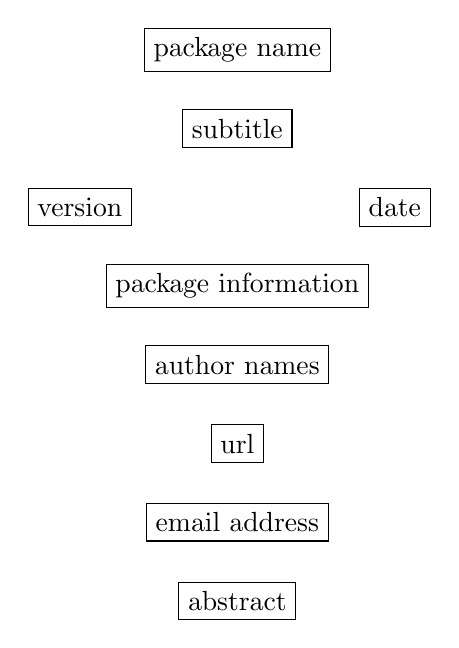
\begin{tikzpicture}
    \node[draw] at (0,0) {package name} ;
    \node[draw] at (0,-1) {subtitle} ;
    \node[draw] at (-2,-2) {version} ;
    \node[draw] at (2,-2) {date} ;
    \node[draw] at (0,-3) {package information} ;
    \node[draw] at (0,-4) {author names} ;
    \node[draw] at (0,-5) {url} ;
    \node[draw] at (0,-6) {email address} ;
    \node[draw] at (0,-7) {abstract} ;
  \end{tikzpicture}
  \caption{Schematic sketch of the title page.}
  \label{fig:titlepage}
\end{figure}

\subsection{Predefined Preamble}\label{sec:preamble}

It is posssible to load a part of my standard preamble automatically by
passing an option as class option.
\begin{options}
  \opt{load-preamble}
    Class option that preloads part of my custom preamble.
\end{options}

Using the option will include the following code:

\begin{sourcecode}
  \RequirePackage[oldstyle]{libertine}
  \RequirePackage{libertinehologopatch}% not on CTAN, yet!
  \RequirePackage[supstfm=libertinesups]{superiors}
  \RequirePackage{microtype}
  \RequirePackage[scaled=.83]{beramono}
  \RequirePackage{fnpct}
  \RequirePackage[english]{babel}
  \renewcommand*\othersectionlevelsformat[3]{%
    \textcolor{cnltxample}{#3\autodot}\enskip}
  \renewcommand*\partformat{%
    \textcolor{cnltxample}{\partname~\thepart\autodot}}
  \deffootnote{2em}{1em}{\llap{\thefootnotemark. }}%
\end{sourcecode}

\section{Predefined Colors and Color-Schemes}\label{sec:colors}

%TODO

\printindex

\end{document}
